\chapter{Evaluation}

The evaluation chapter focuses on demonstrating and evaluating the system based on the defined use cases and quality standards mentioned in \autoref{chap:requirements}. 
The main objective is to assess the system's performance, usability, and compliance to the expected standards. 

\section{Demonstration}
In this section, the application as the result of this thesis will be demonstrated. The demonstration will follow the following procedure to show the key features and functionalities.

Firstly, explore the user management functionality within the application. 
In order for the application to function properly, an active user needs to be created.
To create a new user, simply fill in all the required information in the provided input fields and press on the "New User" button.
Once a user is created, it will be automatically set as the current active user.
To update the information, modify the input fields and clicking on the "Update User" button.
Additionally, the option to permanently delete a user profile is available.
\begin{figure}[H]
    \centering
    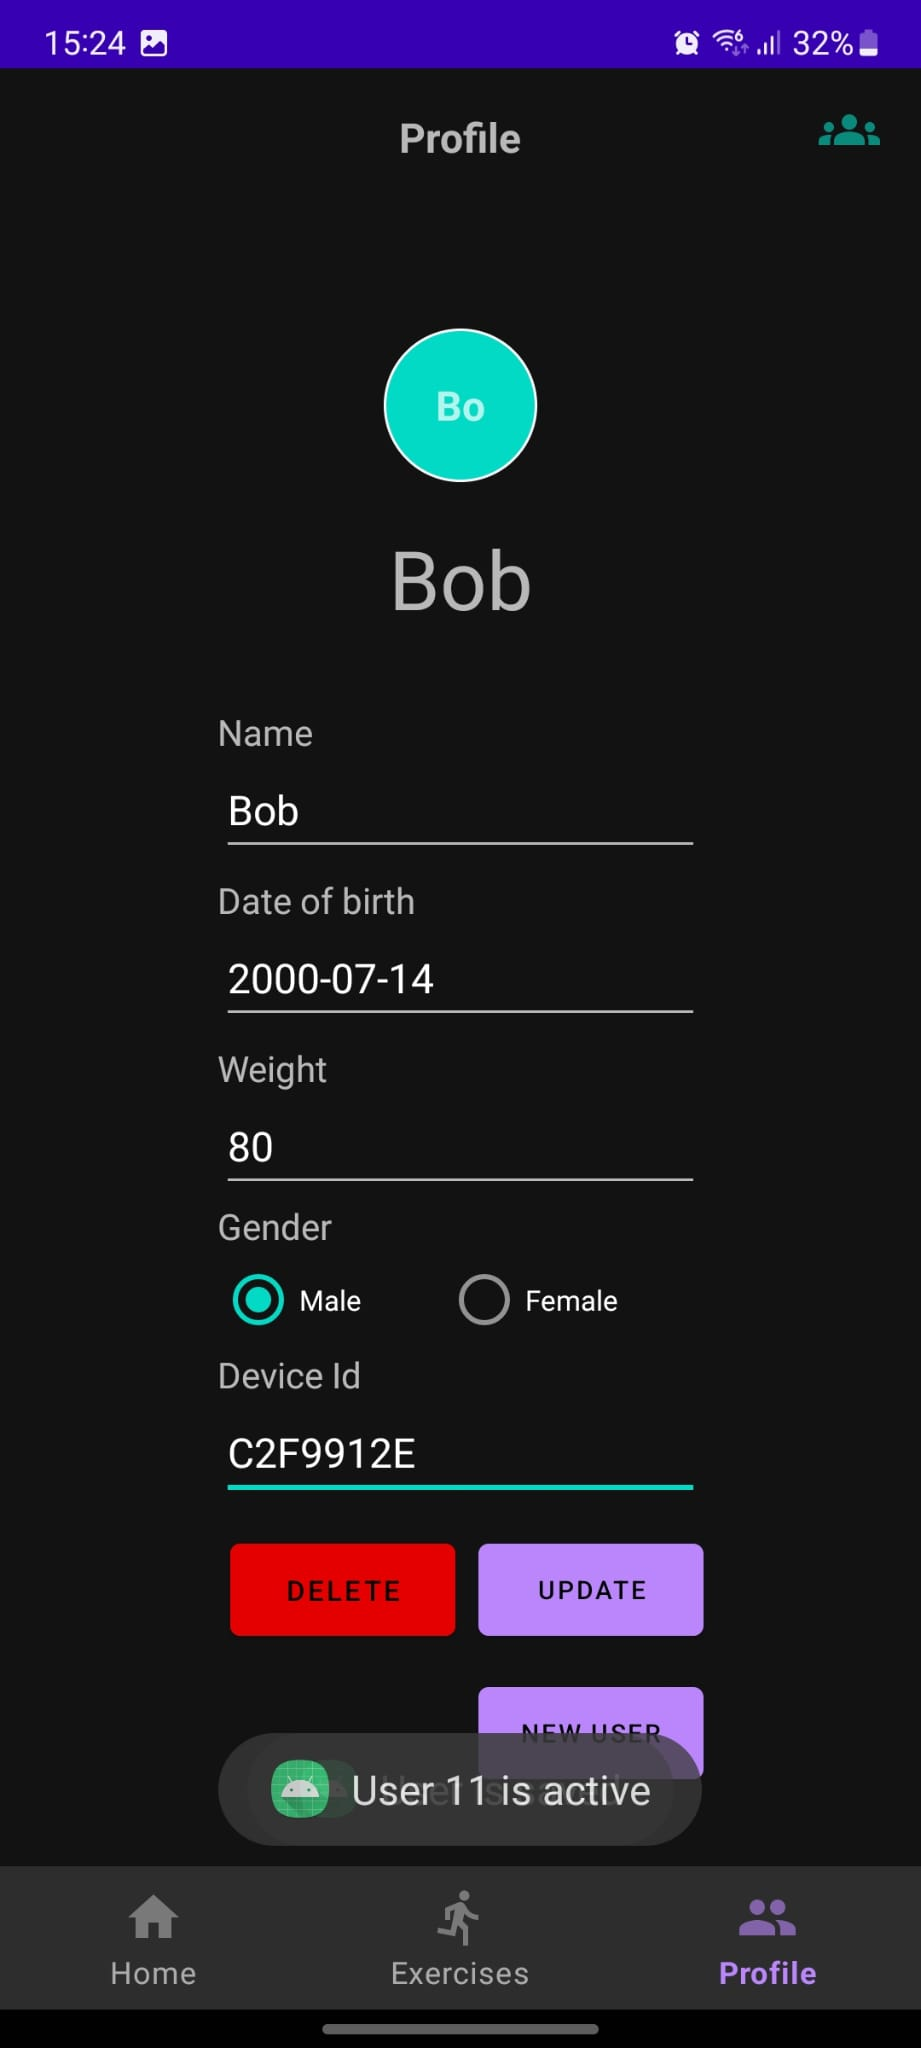
\includegraphics[width=0.5\textwidth]{images/add-new-user.jpeg}
    \caption{Screenshot of successfully adding a new user}
    \label{fig:add-new-user-screenshot}
\end{figure}

Once a user has been successfully added and set active, a connection to the heart rate sensor can be established and heart rate streaming can be started.
Using the bottom navigation, navigate to the home and initiate connection and start heart rate streaming, by simply toggle the switch. 
As the heart rate data is streamed, a dynamic graph will be displayed, providing a visual representation of the user's heart rate.
Furthermore, the user's activity intensity level will be displayed.
\begin{figure}[H]
    \centering
    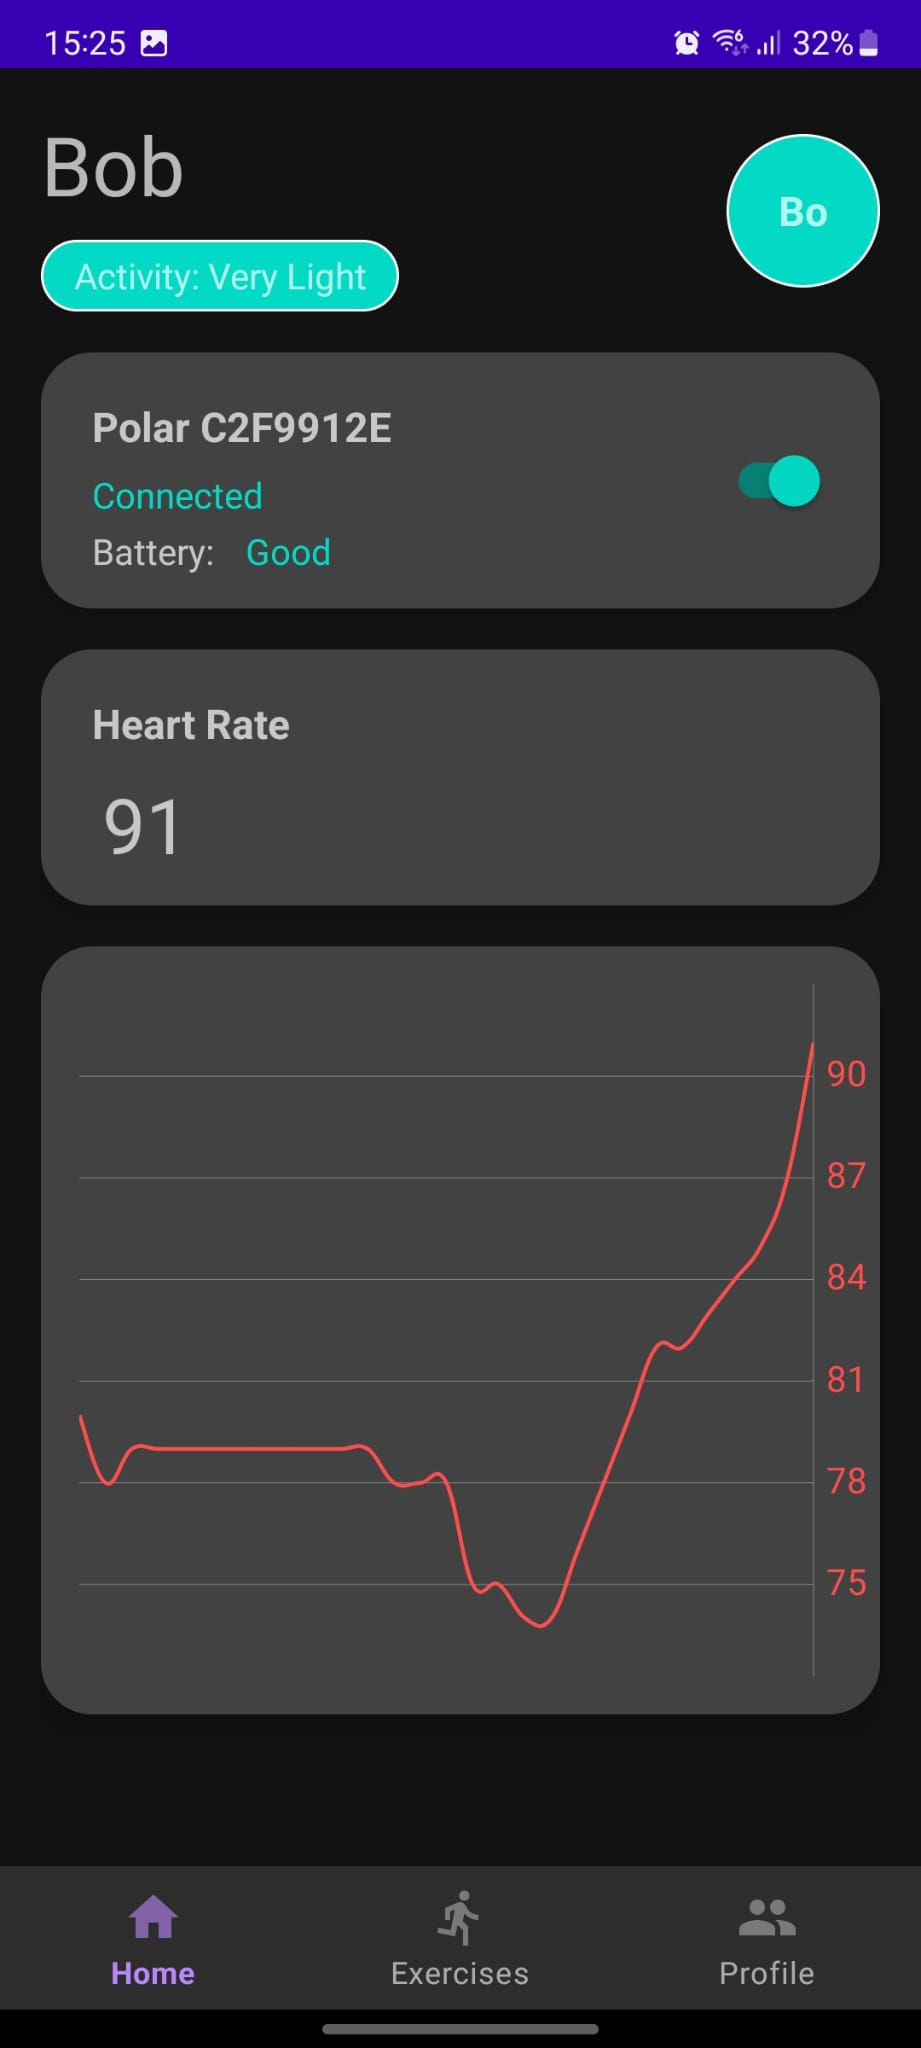
\includegraphics[width=0.5\textwidth]{images/home-sc.jpeg}
    \caption{Screenshot of home page, displaying user's heart rate and activity level}
    \label{fig:home_screenshot}
\end{figure}

After the heart rate streaming has begun, an exercise can be started by navigating to the exercise page and pressing the start button.
The application will then track the exercise progress, including calculating the calories burned. 
To stop the exercise, simply press the stop button. Once an exercise is completed, it will be displayed below, providing a record of the user's workout history.
\begin{figure}[H]
    \centering
    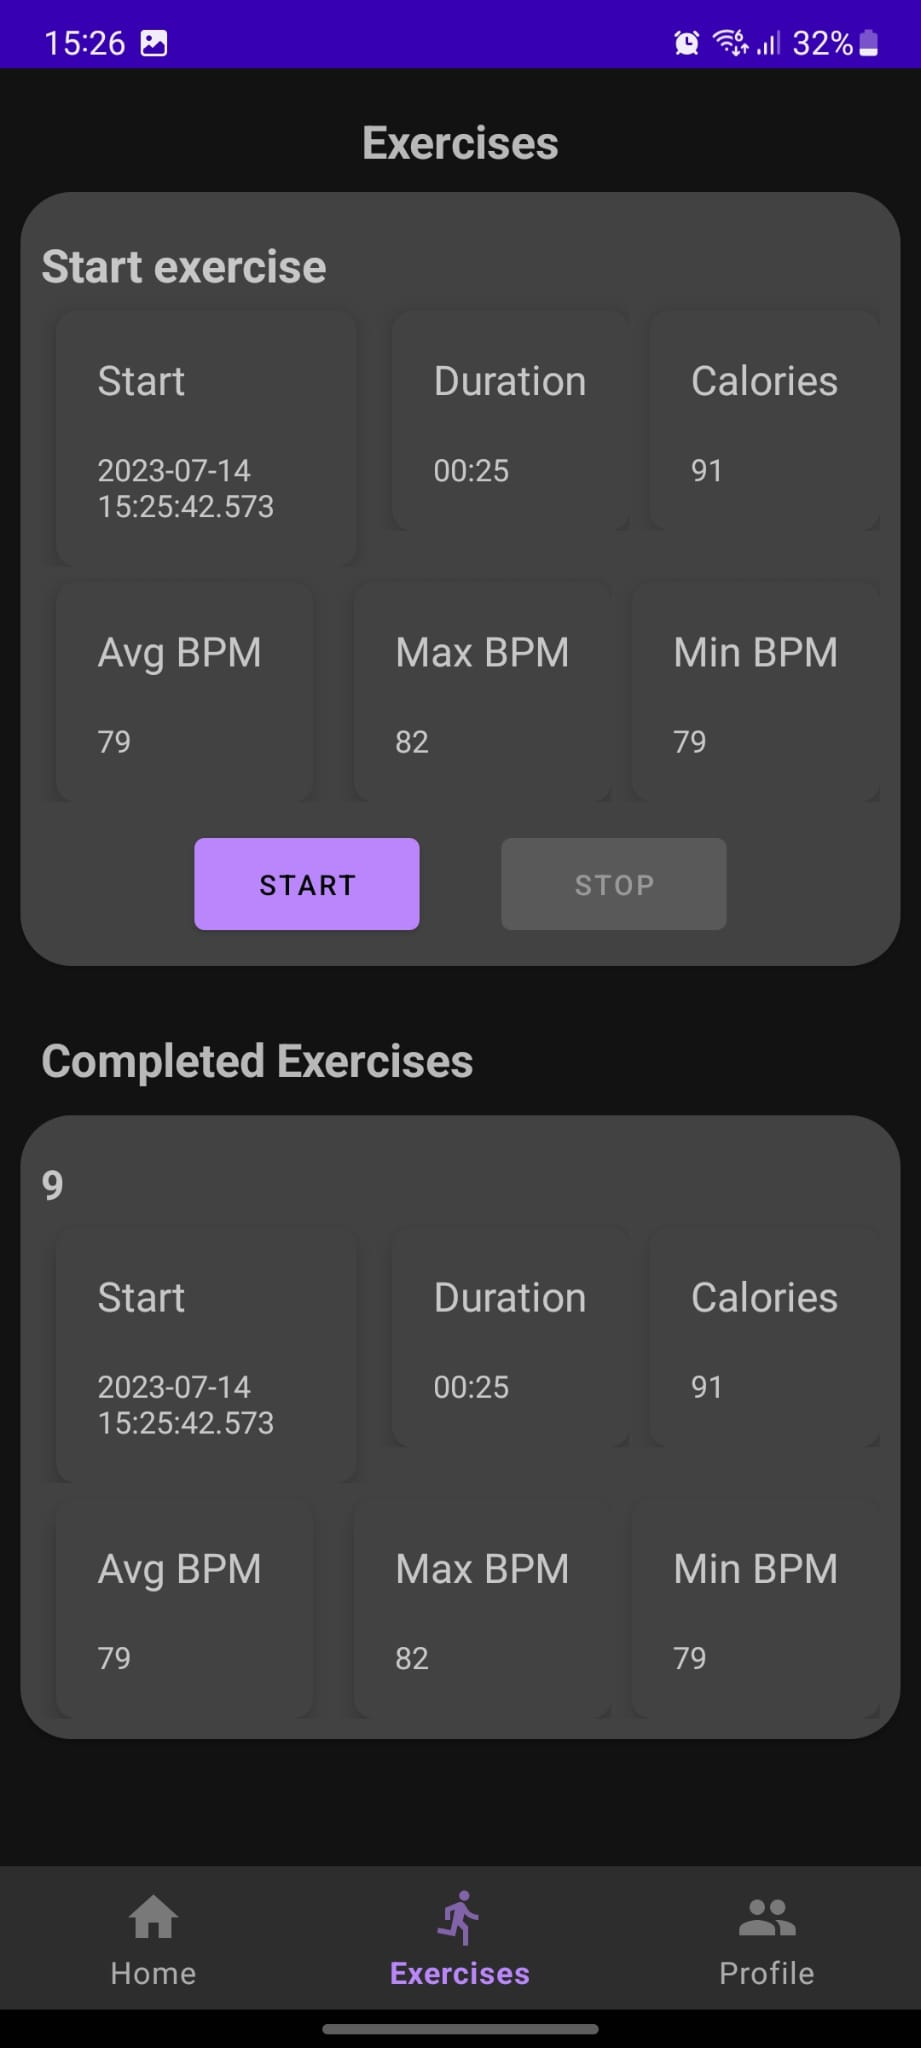
\includegraphics[width=0.5\textwidth]{images/exercise-tracking-sc.jpeg}
    \caption{Screenshot of exercise page, displaying user's exercise information}
    \label{fig:exercise_screenshot}
\end{figure}



\section{Evaluation}
The fulfillment of the requirements and standards outlined in \autoref{chap:requirements} should be used as an assessment metric to determine if the system and its functions have achieved their primary purpose in alignment with the goals of this thesis. 
The implementation of each user story detailed in \autoref{chap:use_case} is listed in \autoref{tab:user_story_and_assessment}.
\clearpage
\begin{longtable}{p{0.5\textwidth} p{0.5\textwidth}}
    \label{tab:user_story_and_assessment}\\

    \caption{Implementation of the user stories}\\
        \hline
        \textbf{User Story} & \textbf{Implementation} \\
        \hline
        As a health-oriented user, I want to monitor my cardiovascular activity. & Provides a functionality to control connection to the heart rate sensor and start heart rate data streaming. The received heart rate data is visualized in form of a line graph.\\
        \hline
        As a physically active individuals, I want to track my current activity so that I can make adjustments to my physical activities. & Processes the received heart rate data to show the intensity of the user's current activity and displays it on the user interface.\\    
        \hline
        As a fitness enthusiast, I want to know the number of calories burned in my exercises. This allows me to keep track of my progress and make adjustments to my exercises. & Provides a functionality to start and stop user exercise and the burned calories will be automatically calculated. The completed exercises are also displayed in the user interface.\\
        \hline
        As a user of the application who is concerned about data privacy, I want to be able to manage and control my user profile easily. & Provides an interface to add, update, and delete user data.\\
        \hline
\end{longtable}

The implementation of Bluetooth Low Energy to establish connection between the application and the heart rate sensor ensures efficient battery usage while providing real-time streaming of heart rate data. 
The application processes the received heart rate data and transforms it into an interactive line graph. 
However, it would be beneficial to include time information in the graph to provide a clearer understanding of the heart rate history.

Furthermore the application determines the user's physical activity intensity level based on the received heart rate data, allowing the users to monitor their activity intensity level.

Moreover, the exercise tracking feature provides user the ability to track their own exercise. The application displays the duration, heart rate information, time and calories burned during the exercise.
However, the application might not provide the most precise estimation of calories burned during exercises as the formula used for the calculation is based on an article published in 2005\autocite{keytel2005energy}.     

From the user management perspective, the application provides users with full control over their own data, allowing them to add, update, and delete their own data.
This feature improves the overall user experience by providing control and ownership over their data.

Additionally, the application should be assessed based on the standards described in \autoref{tab:qualitystandard} to determine the quality of the application.
\newline
\newline
\begin{longtable}{p{0.2\textwidth} p{0.2\textwidth} p{0.5\textwidth}}
    \label{tab:qualitystandard_evaluation}\\

    \caption{Evaluation of the result application based on the standard described in \autoref{tab:qualitystandard}}\\

        \hline
        \textbf{ID} & \textbf{Relevance} & \textbf{Completion} \\
        \hline
        \multicolumn{3}{@{}l}{\textbf{Navigation}} \\
        VX-N1 & less important & complete, the app supports back button navigation.\\
        VX-N2 & less important & complete, the app supports gesture navigation.\\
        VX-N3 & important & complete, the \emph{fragments} will retrieve data at the start of their lifecycle. \\

        \multicolumn{3}{@{}l}{\textbf{UI and Graphics}} \\
        VX-U1 & less important & incomplete\\
        VX-U3 & less important & incomplete\\
  
        \multicolumn{3}{@{}l}{\textbf{Visual quality}} \\
        VX-V1 & less important & complete, icons are implemented using vector drawables.\\
        VX-V3 & not important & complete, the app supports dark theme using Material Design.\\
        
        \multicolumn{3}{@{}l}{\textbf{Accessibility}} \\
        VX-A1 & less important & incomplete, there are some targets smaller than 48dp\\
        VX-A2 & important & complete, the app display are easily readable.\\
        
        \multicolumn{3}{@{}l}{\textbf{Background Service}} \\
        FN-B1 & important & complete, there are restriction for \texttt{ExerciseService} and \texttt{ConnectionService}. Only one instance of each services can run at the same time.\\

        \multicolumn{3}{@{}l}{\textbf{Stability}} \\
        PS-S1 & very important & complete, the application does database transactions in a coroutine.\\

        \multicolumn{3}{@{}l}{\textbf{Performance}} \\
        PS-P1 & important & incomplete\\
        
        \multicolumn{3}{@{}l}{\textbf{Permissions}} \\
        SC-P1 & important & complete.\\
        SC-P4 &  important & complete, at the first time the app starts, permissions are asked and explained the usage. \\
        SC-P5 & important & incomplete\\
        
        \multicolumn{3}{@{}l}{\textbf{Data \& Files}} \\
        SC-DF1 & important & complete, all of the data are stored in local database.\\
        SC-DF2 & important & complete, logging only contains the id of the entities.\\
        SC-DF3 & not important & complete.\\

        \hline
\end{longtable}